  \subsection{Calibración del dial del Generador de Barrido}
    El generador de barrido viene provisto de un cristal externo, el cual oscila a una frecuencia de $5,5~MHz$.
    De esta forma, dicho cristal puede ser utilizado para calibrar el dial del generador de marcas. Para saber
    si se encuentra calibrado, simplemente se conecta el cristal y se lleva al generador de marcas a la frecuencia
    antes mencionada, y por medio de un pequeño parlante, debería escucharse un sonido intenso. La prueba puede
    hacerse también con frecuencias que son armónicos de la de oscilación del cristal, como por ejemplo, un 
    valor de $11~MHz$. Lo mencionado fue puesto a prueba, como puede verse en la Figura~\ref{fig:CalibDial},
    y el generador se encontraba correctamente calibrado.
    
    Para realizar este paso, con la perilla \textbf{Freq. Range} se debe seleccionar la banda \textbf{A} (2 a 6 [MHz]), y 
    con el mando \textbf{Mod. Select} se elige \textbf{RF/Calib.}.

    \begin{figure}[H]
      \centering
      \begin{subfigure}[ht]{0.48\textwidth}
        \frame{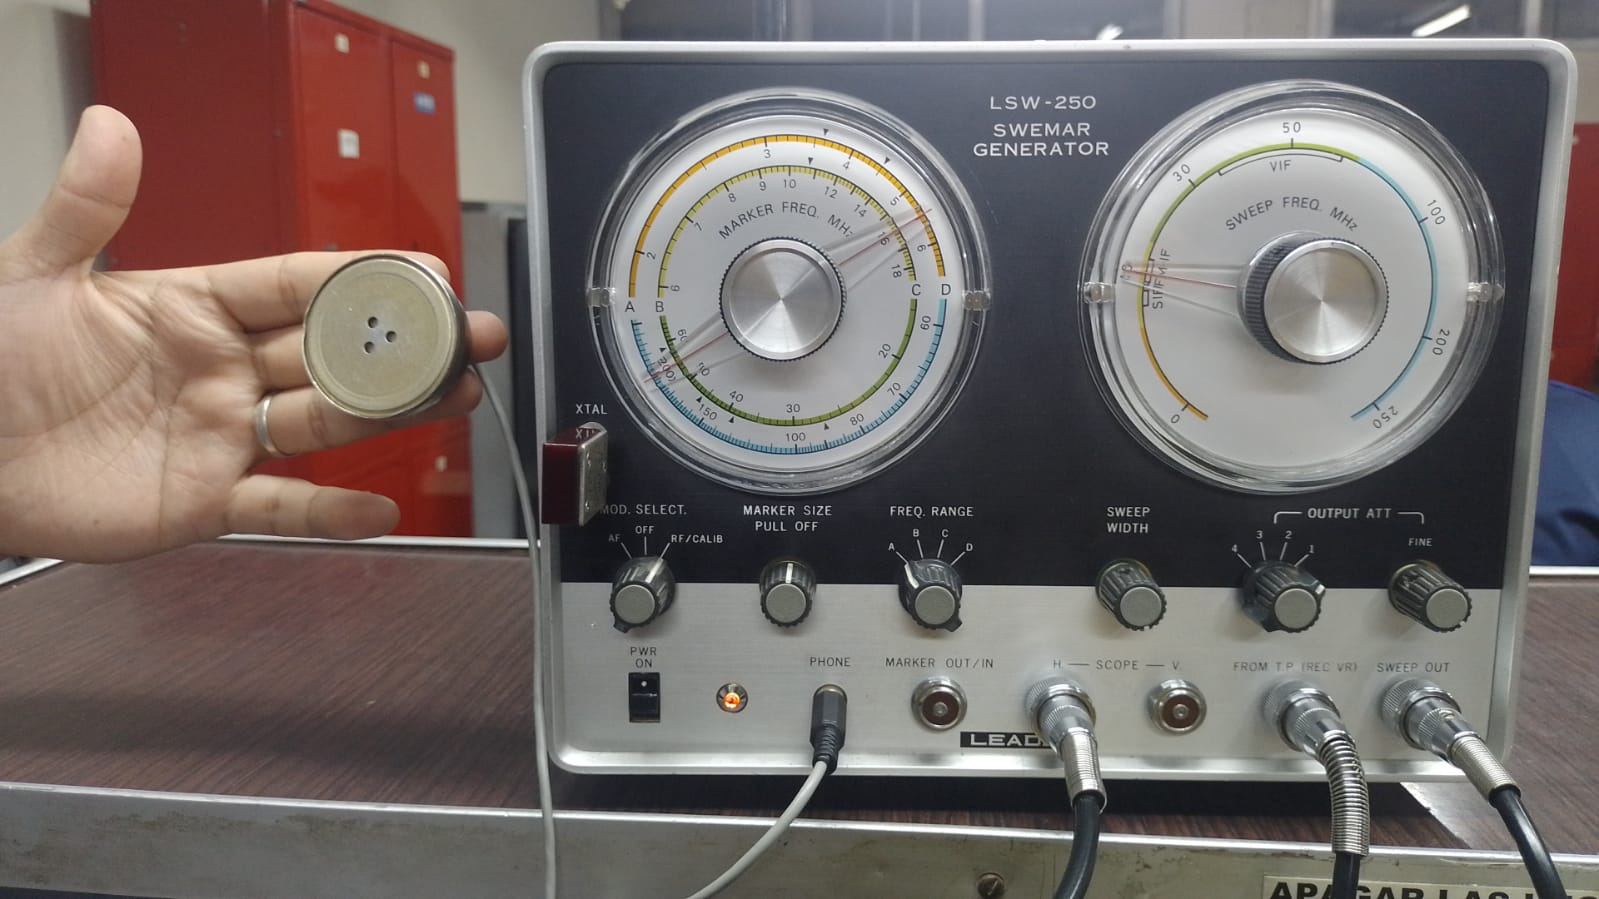
\includegraphics[width=\textwidth]{Imagenes/ActividadPractica/CalibracionDial/Exp1_CalibracionConAudifono5.5MHz.jpeg}}
        \caption{Calibración a $5,5~MHz$.}
        \label{fig:Calib5_5MHz}
      \end{subfigure}
      \hfill 
      \begin{subfigure}[ht]{0.48\textwidth}
        \frame{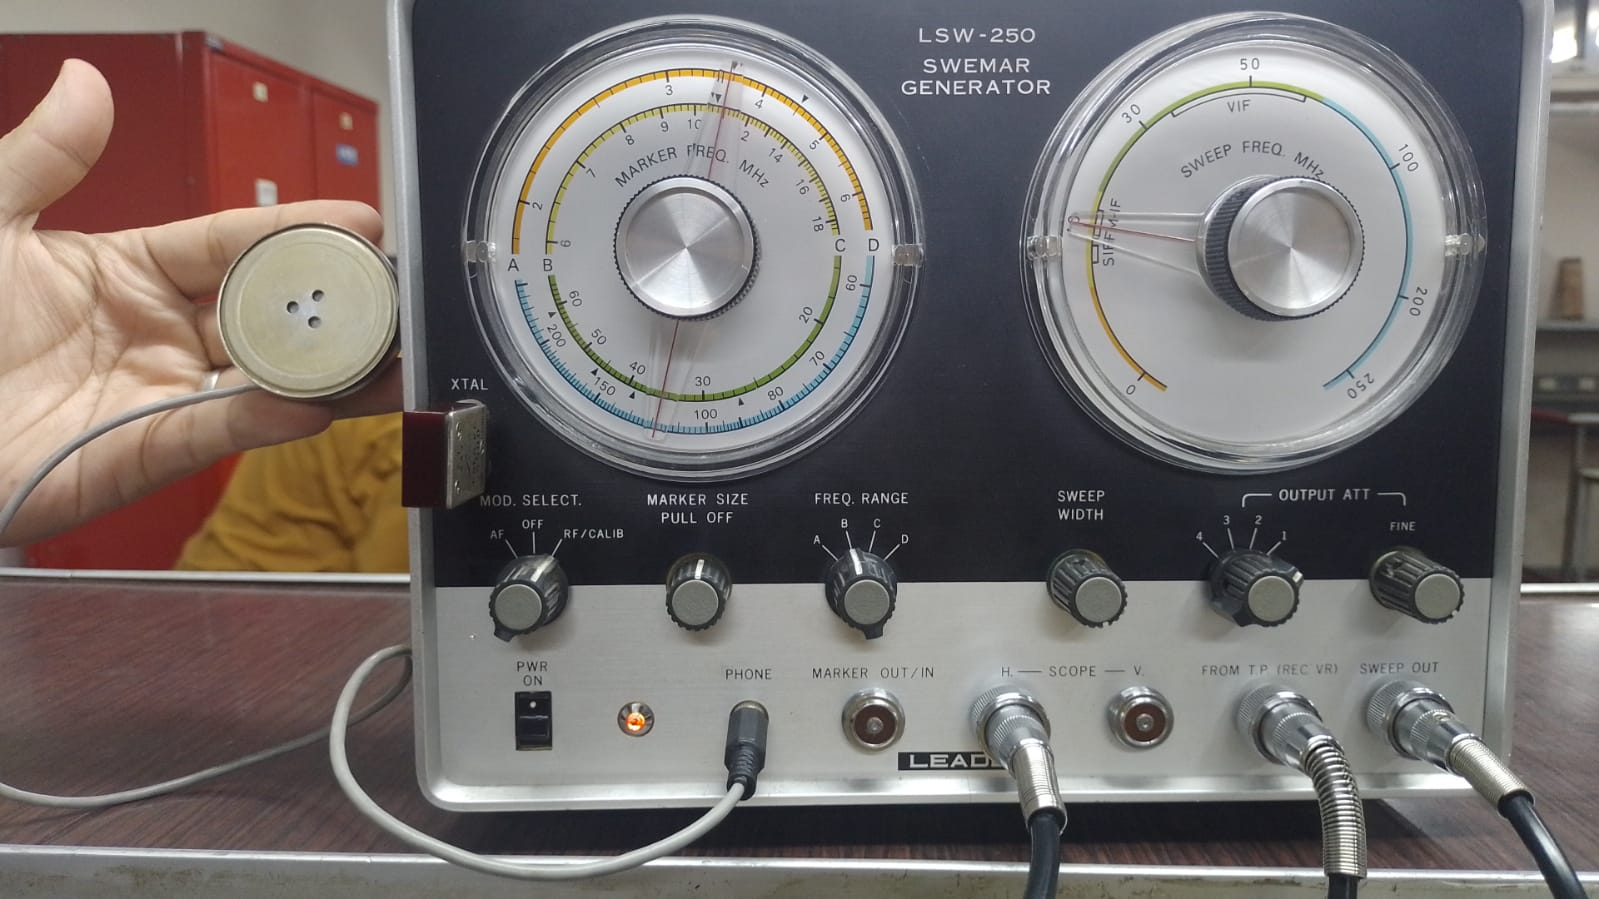
\includegraphics[width=\textwidth]{Imagenes/ActividadPractica/CalibracionDial/Exp1_CalibracionConAudifono11Mhz.jpeg}}
        \caption{Calibración a $11~MHz$.}
        \label{fig:Calib11MHz}
      \end{subfigure}

      \caption{Calibración del dial.}
      \label{fig:CalibDial}
    \end{figure}

    Una vez realizada la calibración, se procede a ver determinadas señales del generador de barrido y marcas. La salida
    identificada como \textbf{H} es la que genera el canal horizontal del espectro de frecuencias que puede ser visto
    en el osciloscopio. Dicha salida se conecta al \textbf{canal 1} del osciloscopio, y, como es de esperarse, la señal debe 
    tener una forma triangular.

    Luego, la salida \textbf{SWEP OUT} del generador es la que genera el barrido en frecuencia. Por lo tanto, si la misma
    es conectada al \textbf{canal 2} del osciloscopio, entonces lo que debe verse es una señal modulada en frecuencia, la cual
    coincide con la pendiente de subida del canal horizontal (el barrido es realizado en un solo sentido). 

    En la Figura~\ref{fig:SeñalDisparoySeñalFM} se pueden ver las dos señales mencionadas anteriormente.

    \begin{figure}[H]
      \centering
      \frame{\includegraphics[width=0.6\textwidth]{Imagenes/ActividadPractica/CalibracionDial/Exp1_SeñalesDisparoYModulada.jpg}}
      \caption{Señal de disparo y modulada en frecuencia.}
      \label{fig:SeñalDisparoySeñalFM}
    \end{figure}

    Por último, si se varía la perilla \textbf{SWEEP WIDTH} puede apreciarse ciertos cambios en la señal modulada en frecuencia.
    El efecto que tiene dicha perilla se ve reflejado en la amplitud de la onda modulada en frecuencia, por lo cual, se debe
    tener especial atención al ancho de banda del osciloscopio para poder visualizar bien esta onda. En la 
    Figura~\ref{fig:EfectoDeAnchoDeBarrido} se pueden ver estas variaciones.


    \begin{figure}[H]
      \centering
      \begin{subfigure}[ht]{0.48\textwidth}
        \frame{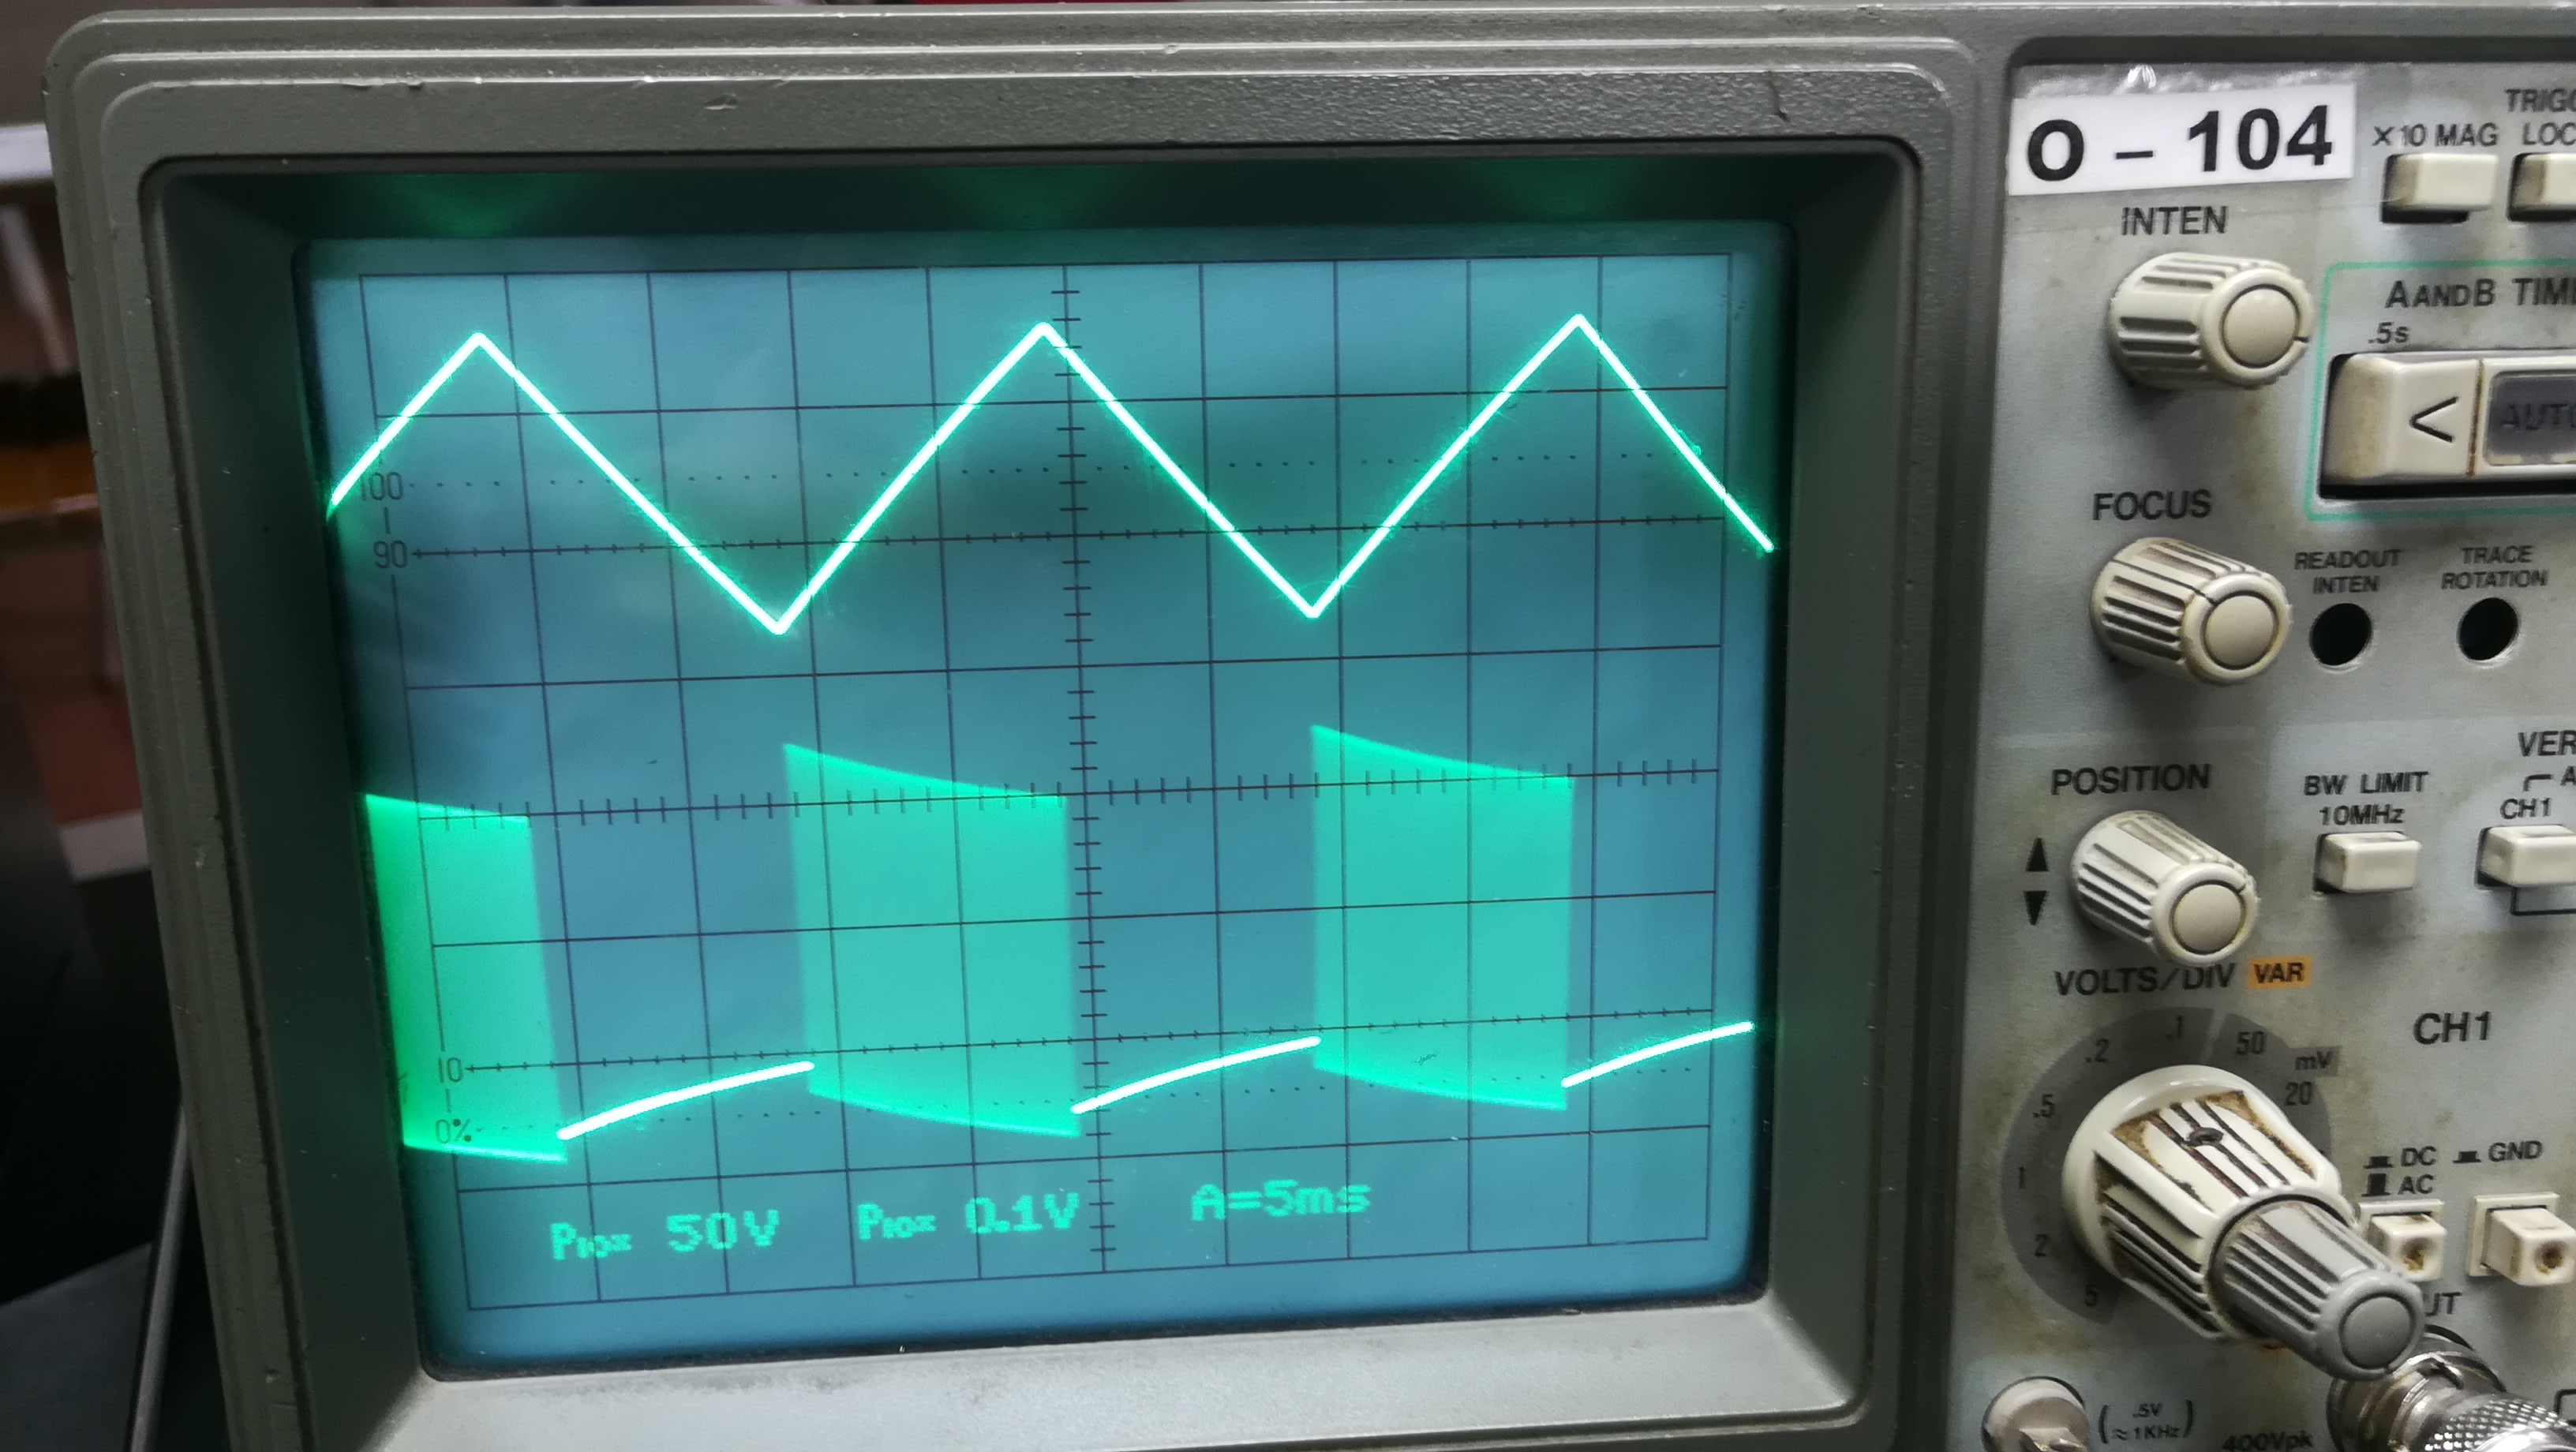
\includegraphics[width=\textwidth]{Imagenes/ActividadPractica/CalibracionDial/Exp1_SweepWidthMinimo.jpg}}
        \caption{Ancho de barrido mínimo.}
        \label{fig:AnchoBarridoMin}
      \end{subfigure}
      \hfill 
      \begin{subfigure}[ht]{0.48\textwidth}
        \frame{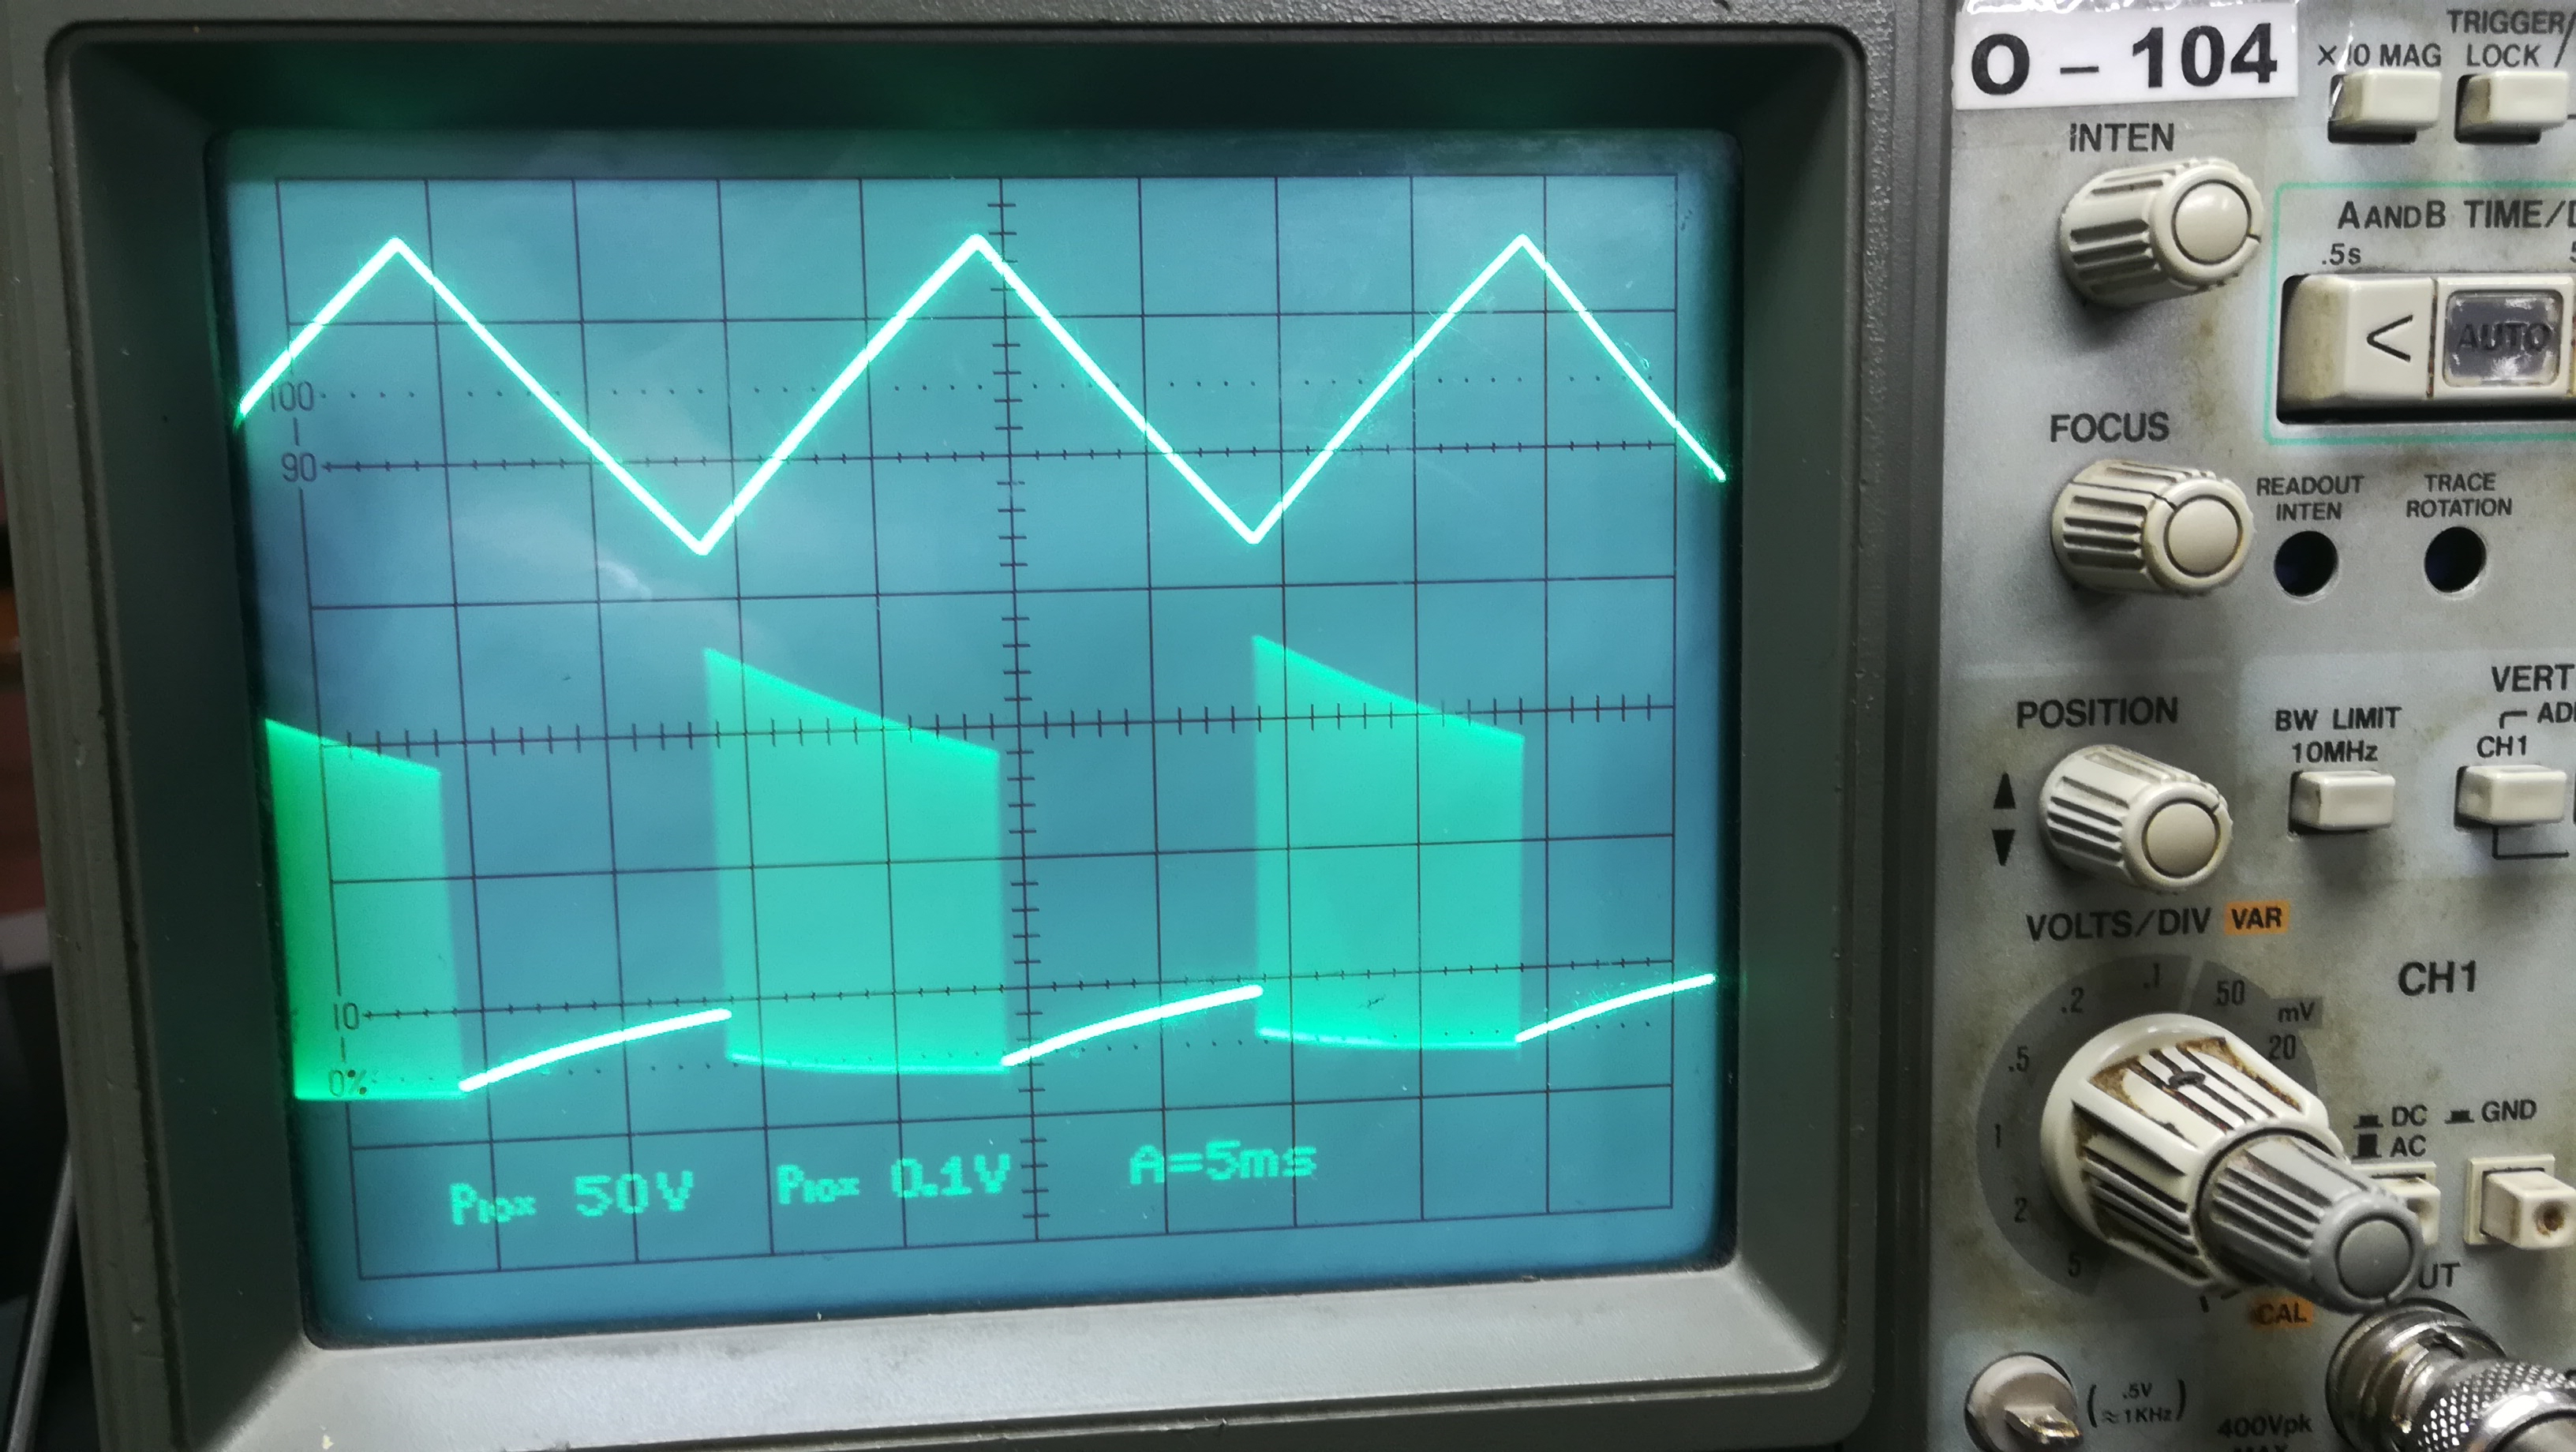
\includegraphics[width=\textwidth]{Imagenes/ActividadPractica/CalibracionDial/Exp1_SweepWidthMedio.jpg}}
        \caption{Ancho de barrido medio.}
        \label{fig:AnchoBarridoMed}
      \end{subfigure}
      \hfill 
      \begin{subfigure}[ht]{0.48\textwidth}
        \frame{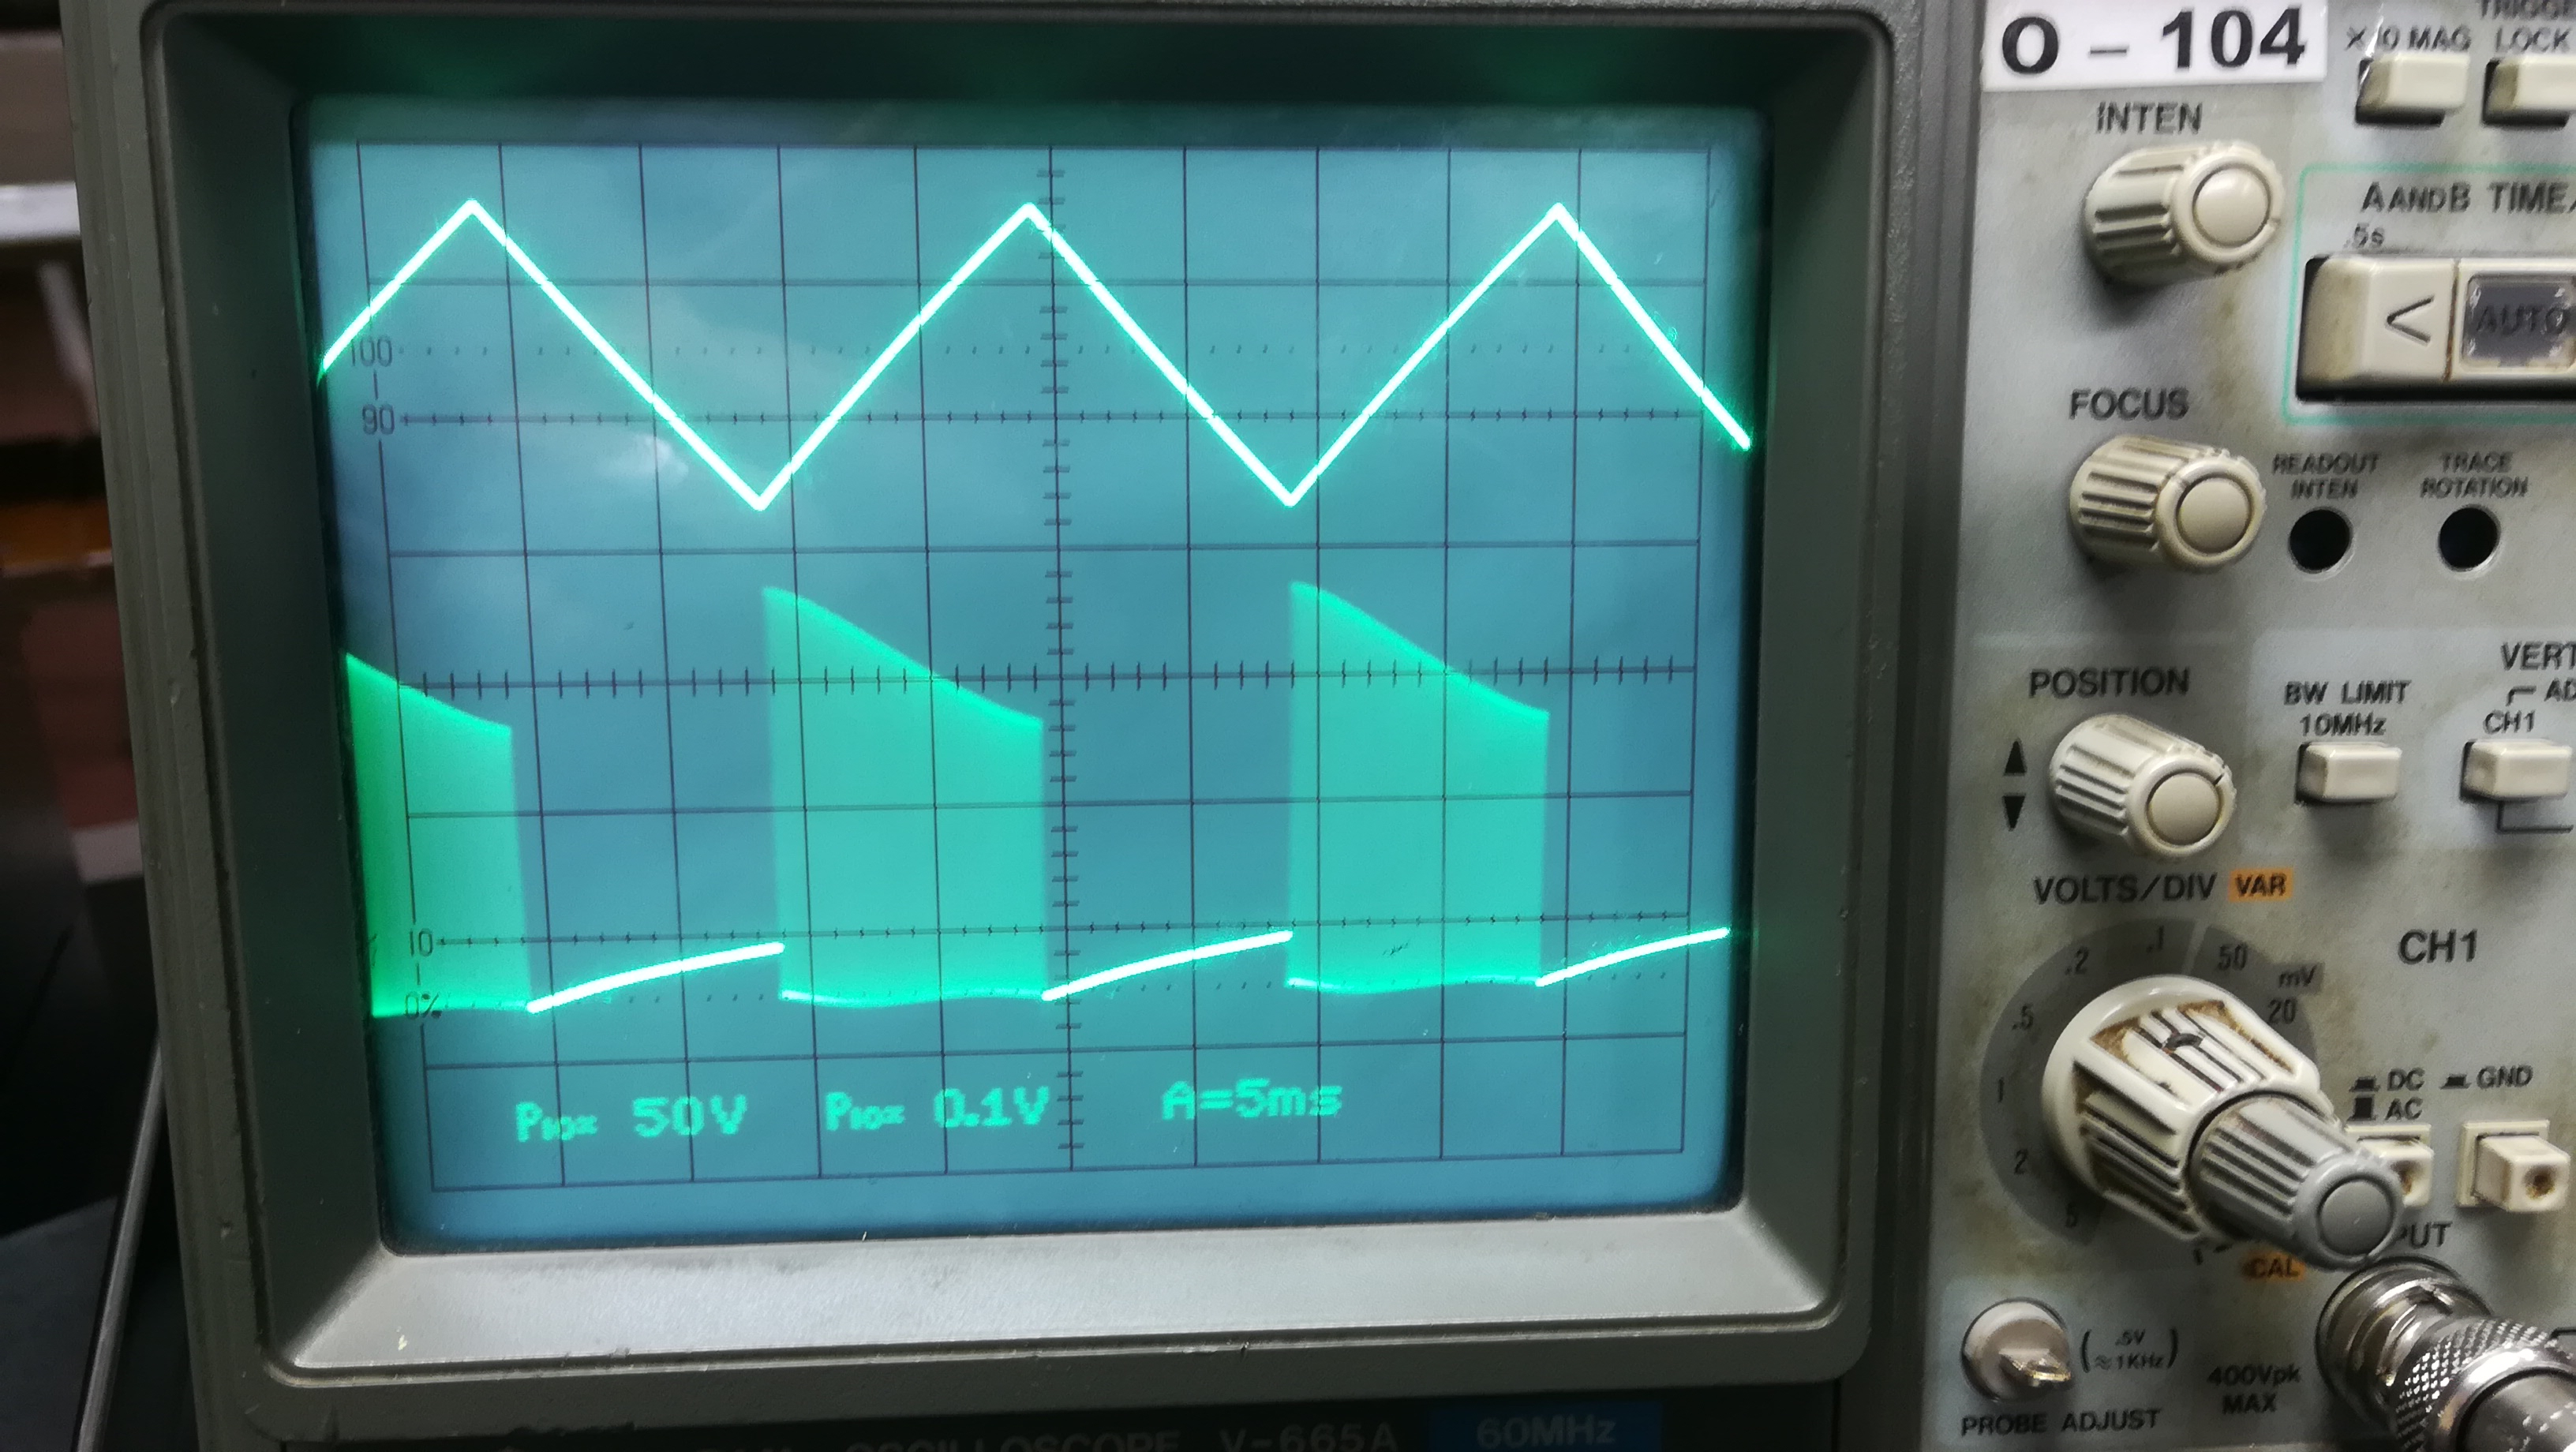
\includegraphics[width=\textwidth]{Imagenes/ActividadPractica/CalibracionDial/Exp1_SweepWidthMaximo.jpg}}
        \caption{Ancho de barrido máximo.}
        \label{fig:AnchoBarridoMax}
      \end{subfigure}

      \caption{Efectos sobre la señal de FM por el ancho de barrido.}
      \label{fig:EfectoDeAnchoDeBarrido}
    \end{figure}
